\section{Discussion}

\label{sec:discussion}It is well known that the accretion processes
of black holes and the resultant energy deposition into the host galaxy
are necessary ingredients in the evolution of galaxies over cosmic
time. Although we do not understand the causal relationship between
the black hole and its host galaxy, our ability to constrain the mechanisms
responsible are derived principally from simulations of the phenomena.
Using the Illustris-2 simulation, we are able for the first time to
quantify the growth and evolution of supermassive black holes in a
cosmological simulation at the resolution of \textbf{XXX }${\rm M_{\odot}}$.
Using these high-resolution simulation results, we have modelled both
the x-ray and radio luminosities as a function of black hole mass
over the full range present in the Illustris-2 simulation.

In Figure \ref{fig:bhpop_hist2d}, we find that the accretion rate
of black holes with masses less than the median mass of $\mathbf{XXX}{\rm M}_{\odot}$
exhibit accretion rates that differ by \textbf{N} orders of magnitude.
Further, \textbf{XXX\%} exhibit accretion rates less than $10^{-10}\,{\rm M_{\odot}s^{-1}}$
indicating that, on the average, a black hole must accrete for $\mathbf{XX}\,{\rm Gyrs}$
to achieve the median mass. These accretion rates are too low to account
for their masses at $z=0$. For example, a typical low-mass ($10^{7}M_{\odot}$)
black hole accretes at approximately $10^{-12}M_{\odot}s^{-1}$ at
$z=0$. At this rate, such a black hole could only yields a mass of
$\sim10^{5}M_{\odot}$ over the simulation time. Although the high-mass
black holes have generally larger accretion rates in excess of $\dot{M}\approx10^{-10}M_{\odot}s^{-1}$,
the same calculation yields masses of $\sim10^{7}M_{\odot}$ compared
to the actual mass of $\sim10^{9}M_{\odot}$ attained over the simulation
time. This implies that the accretion rates for most of the black
holes in the simulation were likely much larger in the past. This
is consistent with the notion that black hole accretion rates are
tied to the gas fraction in galaxies which was larger at higher redshift.
\textbf{Can we find out when the BH was seeded? I want to make a plot
of seed time vs mass to make this more concrete. Is the linear relation
between mass and $\dot{M}$ known either empirically or from theory?}

\textbf{Talk about Figure 5.}

\begin{figure}
\begin{centering}
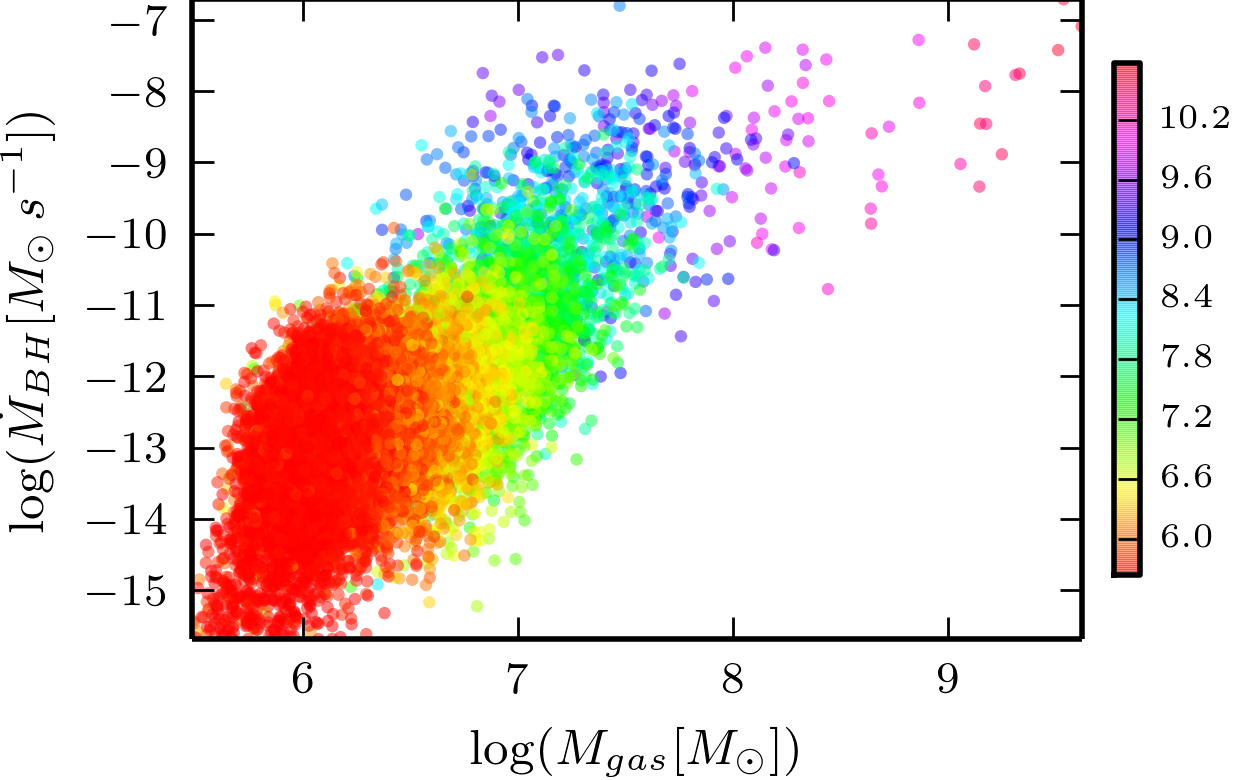
\includegraphics[scale=0.75]{Figures/Mdot_vs_Mgas}
\par\end{centering}

\protect\caption{\label{fig:Mdot_vs_Mgas}Black hole accretion rate of as a function
of the total gas mass in each subhalo for our sample. Colors correspond
to black hole mass. All masses are in units of $\log\left(M_{\odot}\right)$
and the accretion rate is in units $\log\left(M_{\odot}yr^{-1}\right)$.}
\end{figure}
